\documentclass{article}

\usepackage{fancyhdr}
\usepackage[T1]{fontenc}
\newcommand{\changefont}[3]{\fontfamily{#1} \fontseries{#2} \fontshape{#3} \selectfont}

\usepackage{listings}
\usepackage{color}
\usepackage{hyperref}
\usepackage{graphicx}
\graphicspath{{}}

\definecolor{dkgreen}{rgb}{0,0.6,0}
\definecolor{gray}{rgb}{0.5,0.5,0.5}
\definecolor{orange}{rgb}{0.7,0.7,0}
\definecolor{lightgray}{rgb}{0.92,0.92,0.92}
\definecolor{mauve}{rgb}{0.58,0,0.82}

\lstset{frame=none,
  language=Python,
  aboveskip=3mm,
  belowskip=3mm,
  showstringspaces=false,
  columns=flexible,
  basicstyle={\small\ttfamily},
  numbers=none,
  backgroundcolor=\color{lightgray},
  numberstyle=\color{orange},
  keywordstyle=\color{mauve},
  commentstyle=\color{gray},
  stringstyle=\color{dkgreen},
  breaklines=true,
  breakatwhitespace=true,
  tabsize=3
}




% change title and date every week
\title{BPP Exercise 1 - print("Hello World!")}
\author{A. Hain, M. Nipshagen}
\date{09.04.2018, 8:00}

\makeatletter
\let\thetitle\@title
\let\theauthor\@author
\let\thedate\@date
\makeatother

% header and foot
\pagestyle{fancy}
\fancyhf{}
\fancyhead[L]{\thetitle}
\fancyhead[C]{}
\fancyhead[R]{\theauthor}
\renewcommand{\headrulewidth}{0.4pt}
\fancyfoot[L]{Due: \thedate}
\fancyfoot[R]{\thepage}
\renewcommand{\footrulewidth}{0.4pt}


\begin{document}

The deadline for this exercise sheet is \textbf{Monday, \thedate.}

% ----- PREAMBLE -----
\section*{Some words before we start...}
Welcome to the first exercise! Please submit your solutions to your group's folder
on Stud.IP by the deadline each week. So in case you have not joined a group yet,
please do so now. Though we strongly recommend that every group member solves all
exercises on their own, please upload only one solution per group. We prefer if
you put all your files into a .zip archive and upload this to your folder but
uploading them separately is also fine.\\
So without further ado - let's start!

% ------ INSTALLATION INSTRUCTIONS -----
\section{Installing Python}
First, of course, you need to install Python. We recommend that you use Miniconda
which is a package management system and makes managing a Python installation easy.

\begin{itemize}
\item Download Miniconda from: \href{conda.io/miniconda.html​}{conda.io/miniconda.html}
\item Install and add it to your path (refer to the documentation for that or, if you are having trouble,
come to the walk in session)
\item Then run the following commands in your terminal/command line:
\begin{lstlisting}
conda install pip numpy matplotlib scipy
conda install pandas jupyter scikit-learn scikit-image
\end{lstlisting}
\item You can of course also download Python from the official website and use pip
\end{itemize}


% ----- TASK 1 -----
\section{Hello you!}
To take first steps, we will for now work in the \textit{Python Shell}. To open
it, open your terminal/command line, type in "python" and press return.
It should give you an output similar to this: \\
\changefont{cmtt}{m}{n}\\
Python 3.6.3 |Anaconda, Inc. (default, Oct 15 2017, 03:27:45) [MSC v.1900 64 bit (AMD64)] on win32\\
Type "help", "copyright", "credits" or "license" for more information.\\
{>}>{>}\\
\changefont{cmr}{m}{n}\\
If this is similar to what you're seeing, then you're good to go. (Otherwise, please
check again if Python was installed correctly).\\
Now type the following and hit return:
\begin{lstlisting}
print("Hello World!")
\end{lstlisting}
This will give you the following output:\\
\changefont{cmtt}{m}{n}\\
Hello World!\\
\changefont{cmr}{m}{n}\\
Now modify the statement to create the following outputs:
\changefont{cmtt}{m}{n}
\begin{enumerate}
\item Hi, my name is [your name]!
\item What's up?
\item \textit{Bonus:}\\So what's "Python"?
\item \textit{Bonus:}\\Hello\\World
\end{enumerate}
\changefont{cmr}{m}{n}
To solve the two bonus tasks, you might have to do some googling. It's good to get
used to it right away because programmers have to google. A lot. Therefore, there
will probably be more exercises where we let you ask the internet for help.\\
When you're finished, please write all your statements that succesfully printed
the given sentences into a file and save it using the name \textit{hello.py}.
Feel free to play around with more statements.\\
To exit the Python shell, use the following command:
\begin{lstlisting}
exit()
\end{lstlisting}
\textit{Solution (hello.py):}
\begin{lstlisting}
# from the original print("Hello World!") just change what's inside the brackets
print("Hi, my name is [your name]!")
print("What's up?")

# Bonus
print("So what's \"Python\"?") # use \ to cancel the meaning of "
print("Hello\nWorld") # \n will add a line break
\end{lstlisting}

% ----- TASK 2 -----
\section{Fun with Turtles}
% More shameless copying
In the late 20th century it became very popular to teach programming with a
turtle. Those turtles were little robots that could move around - check one
out \href{https://youtu.be/8wU6NdjTVTA}{here}
\footnote{Check \href{https://en.wikipedia.org/wiki/Turtle_(robot)}{this} for more info.
The concept is still popular today, although turtles are not enough anymore
(\href{https://studio.code.org/s/frozen/stage/1/puzzle/17}{https://studio.code.org/s/frozen/stage/1/puzzle/17})
}
Did you notice that it drew on the sheet of paper? No? Watch again then.\\
Since we can not afford to buy a turtle for everyone, Python allows us to draw
with a virtual turtle. Open your Python interpreter again, as you did in the
previous exercise.\\
\textit{Note for Windows users:} Please use this command instead this time:
\begin{lstlisting}
python -i
\end{lstlisting}
To use the turtle, you first have to tell Python that we need it:
\begin{lstlisting}
import turtle
\end{lstlisting}
To show our turtle, use:
\begin{lstlisting}
turtle.shape('turtle')
\end{lstlisting}
You should see a window like this:\\\\
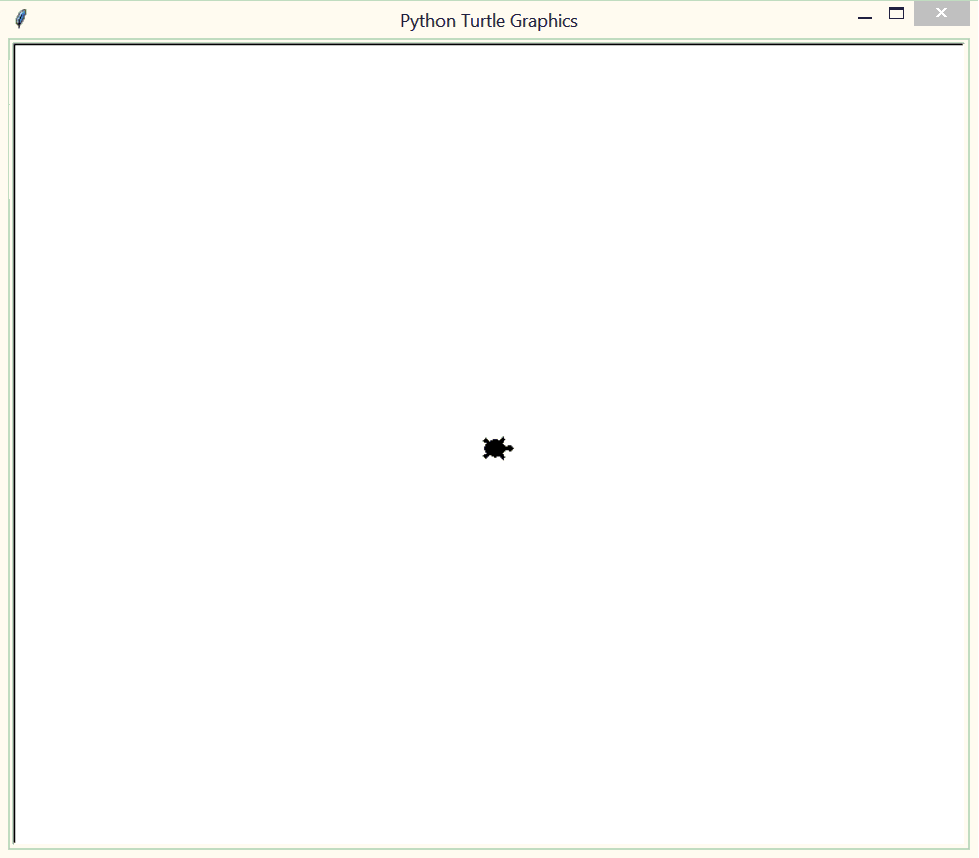
\includegraphics[scale=0.6]{Ex_1_Turtle}\\
Now you can let your turtle move around and draw with the following commands:
\begin{lstlisting}
turtle.forward(100)
turtle.right(90)
turtle.backward(100)
turtle.left(90)
\end{lstlisting}
\textit{Another note for Windows users:} You might notice the turtle window is
sometimes unresponsive in the background. Don't worry - as soon as you're entering
a new command, it will show up in the foreground again.\\\\
If you want to reset what your turtle drew, you can use:
\begin{lstlisting}
turtle.reset()
\end{lstlisting}
In Germany little kids learn to draw the \textit{Haus vom Nikolaus} (St. Nicholas' house)
in one stroke. It looks like this:\\
\begin{center}
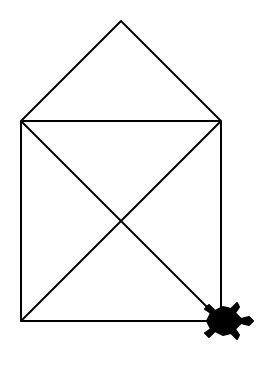
\includegraphics[scale=1]{Ex_1_Nicholas}
\end{center}
Can you give your turtle commands to draw something like this?\\
Store your successful commands in a file names \textit{nicholas.py} for your submission.\\\\
\textit{Solution (nicholas.py):}
\begin{lstlisting}
import turtle

turtle.shape('turtle')

# left edge
turtle.left(90)
turtle.forward(100)

# roof
turtle.right(45)
turtle.forward(70.71)
turtle.right(90)
turtle.forward(70.71)
turtle.right(135)
turtle.forward(100)

# cross and right edge
turtle.left(135)
turtle.forward(141.42)
turtle.right(45) # !
turtle.backward(100)
turtle.right(45)
turtle.forward(141.42)

# bottom edge
turtle.left(135)
turtle.forward(100)

# keep the window open (not needed for the homework)
turtle.done()
\end{lstlisting}

\end{document}
